\subsection{Leibniz on Integration: The General Area of a Curve}  

While differentiation described instantaneous motion, both Newton and Leibniz recognized that integration was its inverse which allowed them to compute the area under a curve.  

Newton thought of integration as summing up infinitesimally small changes in position (essentially reconstructing motion from its velocity).  

Leibniz, on the other hand, created the notation we still use today:

\[
\int dy
\]

But unlike Kepler, who used area to study planetary motion, Newton and Leibniz’s methods could describe any curve, anywhere, in any context (i.e. a falling cannonball, a planet, or even a changing economic trend).  

\begin{figure}[H]
\centering
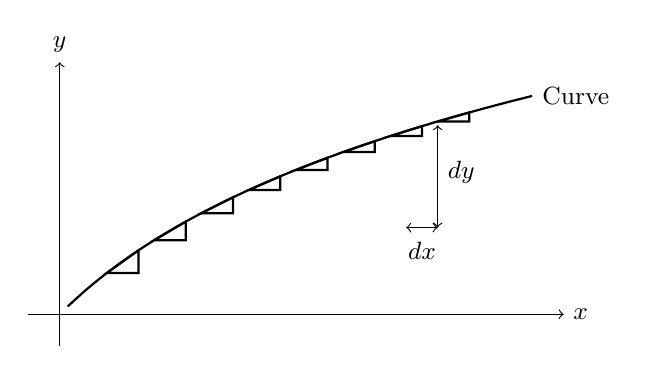
\begin{tikzpicture}[scale=2]
    % Axes
    \draw[->] (-0.2, 0) -- (3.2, 0) node[right] {\small $x$};
    \draw[->] (0, -0.2) -- (0, 1.6) node[above] {\small $y$};

    % Curve (logarithmic function)
    \draw[thick, domain=0.05:3, smooth, variable=\x] plot ({\x},{ln(\x + 1)}) node[right] {\small Curve};

    % Infinitesimal rectangles along the curve
    \foreach \x in {0.3, 0.6, 0.9, 1.2, 1.5, 1.8, 2.1, 2.4} {
        \draw[thick] (\x, {ln(\x + 1)}) -- ({\x + 0.2}, {ln(\x + 1)}) -- ({\x + 0.2}, {ln(\x + 1.2)}) -- cycle;
    }

    % Labels for differentials
    \node at (2.3, 0.4) {\small $dx$};
    \node at (2.55, 0.9) {\small $dy$}; % moved down

    % Arrows showing differential elements
    \draw[<->] (2.2, 0.55) -- (2.4, 0.55);
    \draw[<->] (2.4, 0.55) -- (2.4, 1.2);
\end{tikzpicture}

\vspace{0.5em}
\caption{\small A logarithmic curve with infinitesimal rectangles illustrating the differentials $dx$ and $dy$. The horizontal arrow represents a small fixed change in $x$, while the vertical arrow shows the actual change in $y$ over that interval: $dy = \ln(x+dx+1) - \ln(x+1)$. Since the slope of the function increases with $x$, $dy$ becomes larger for the same $dx$. This reflects the local steepness of the curve and highlights the geometric meaning of the derivative as the ratio $\frac{dy}{dx}$.}
\end{figure}


In Leibniz’s framework, a curve was analyzed through the use of differentials. At any point along the curve, one could consider an infinitesimal triangle formed by two small changes: the horizontal difference, denoted by $dx$, and the corresponding vertical difference, denoted by $dy$. These represented the vanishingly small increments of the variable and its ordinate. The slope of the curve at that point was expressed by the ratio $\frac{dy}{dx}$, which Leibniz interpreted as the differential quotient — the rate at which one quantity changed with respect to another. Though Leibniz focused primarily on these differential relationships, the infinitesimal triangles hinted at a broader method: by summing such differentials along the curve, one could conceive of a total quantity accumulated — an idea that would later be formalized as the integral.

\subsubsection{Leibniz’s View: Infinitesimals, Not Triangles}

Where Newton envisioned geometry in motion, Leibniz saw motion in algebra.

Galileo had shown that a falling body accelerates uniformly — covering distance in proportion to the square of time. But this, for Leibniz, was not merely a fact of nature; it was a structure waiting for notation. He took Galileo’s parabolas and velocities and rewrote them as relations between differentials.


\paragraph{A New Language of Change.} Leibniz conceived of motion as a relation between infinitely small changes. If $s$ is the vertical distance fallen and $t$ is time, then:

\[
\frac{ds}{dt} = v(t)
\]

\begin{figure}[H]
\centering
\begin{tikzpicture}[scale=1.3]

  % Axes
  \draw[->] (0,0) -- (5.5,0) node[right] {$t$ (tempus)};
  \draw[->] (0,0) -- (0,4) node[above] {$s$ (spatium)};

  % Position curve: s(t) = (1/2)gt^2
  \draw[thick,blue,domain=0:5,smooth,samples=100] plot(\x,{0.35*\x*\x});
  \node[blue] at (4.2,3.4) {\footnotesize $s(t) = \frac{1}{2}gt^2$};

  % Tangent line at t = 3
  \coordinate (P) at (3, {0.35*3*3});
  \draw[dashed] (P) -- ++(1, {0.35*2*3}); % Tangent slope = g*t
  \filldraw[blue] (P) circle (1pt);
  \node[above left] at (P) {\scriptsize $s$};

  % Small delta labels
  \draw[<->] (3,0) -- (3,0.2) node[midway,right] {\tiny $dt$};
  \draw[<->] (0,{0.35*9}) -- (0.35,{0.35*9}) node[midway,below] {\tiny $ds$};

  % Slope triangle
  \draw[dashed] (0,0.35*9) -- (0.35,0.35*9);
  \draw[dashed] (0.35,0.35*9) -- (0.35,0);

  % Slope label
  \node at (1.7,2.1) {\scriptsize $\displaystyle \frac{ds}{dt} = v(t)$};

\end{tikzpicture}
\caption{Leibniz's new language of change: motion is built from differentials. At each moment, the derivative $\frac{ds}{dt}$ gives the velocity — an instantaneous rate, not an average triangle.}
\end{figure}


But for Leibniz, this was not a limit — it was a ratio of actual infinitesimal quantities: $ds$ and $dt$. He might write:

\[
ds = v\,dt
\]

where $v$ itself could be changing with time, such as:

\[
dv = g\,dt
\]

\begin{figure}[H]
\centering
\begin{tikzpicture}[scale=1.3]

  % Axes
  \draw[->] (0,0) -- (5.5,0) node[right] {$t$ (tempus)};
  \draw[->] (0,0) -- (0,4) node[above] {$s$ (spatium)};

  % Position curve: s(t) = (1/2)gt^2
  \draw[thick,blue,domain=0:5,smooth,samples=100] plot(\x,{0.35*\x*\x});
  \node[blue] at (4.2,3.4) {\footnotesize $s(t) = \frac{1}{2}gt^2$};

  % Tiny vector at t = 1.5
  \coordinate (P1) at (1.5, {0.35*1.5*1.5});
  \draw[->, thick,green!60!black] (P1) -- ++(0.15, {0.35*2*1.5*0.15});
  \node[right=2pt] at ($(P1)+(0.15,0.2)$) {\scriptsize $ds = v\,dt$};

  % Tiny velocity vector curve below
  \draw[->, thick,red] (1.5,-0.2) -- ++(0.15, {0.7*0.15});
  \node[right=2pt] at (1.7,-0.1) {\scriptsize $dv = g\,dt$};
  \node[below] at (1.5,-0.2) {\scriptsize Velocity};

  % Groundline for velocity strip
  \draw[dashed] (0,-0.2) -- (5.5,-0.2);

  % Visual tiny rectangle to show dt
  \draw[<->] (1.5,-0.35) -- (1.65,-0.35);
  \node[below] at (1.575,-0.35) {\tiny $dt$};

\end{tikzpicture}
\caption{For Leibniz, $ds$ and $dt$ are not vanishing limits, but real infinitesimal quantities. The equation $ds = v\,dt$ expresses how distance accumulates from velocity, and $dv = g\,dt$ shows how velocity itself changes — stacked differentials, not triangles.}
\end{figure}


Here, $g$ is the constant acceleration due to gravity. From this, he would integrate — or, in his words, "sum the differentials":

\[
v = \int g\,dt = g t
\quad \text{then} \quad
s = \int v\,dt = \int g t\,dt = \frac{1}{2}gt^2
\]

Thus, Leibniz derived Galileo’s law not from experiment but from algebra — manipulating symbols like $ds$ and $dt$ as real, albeit infinitesimal, quantities.

\begin{figure}[H]
\centering
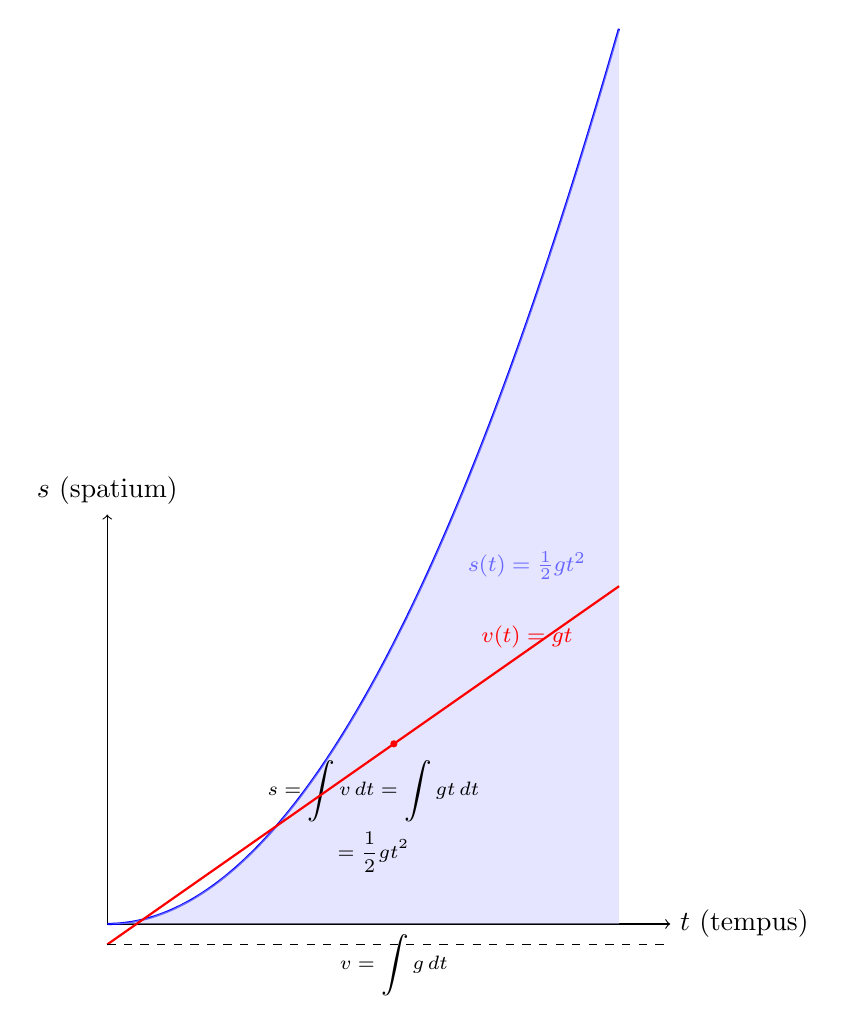
\begin{tikzpicture}[scale=1.3]

  % Axes
  \draw[->] (0,0) -- (5.5,0) node[right] {$t$ (tempus)};
  \draw[->] (0,0) -- (0,4) node[above] {$s$ (spatium)};

  % Position curve: s(t) = (1/2)gt^2
  \draw[thick,blue,domain=0:5,smooth,samples=100] plot(\x,{0.35*\x*\x});
  \node[blue] at (4.1,3.5) {\footnotesize $s(t) = \frac{1}{2}gt^2$};

  % Shaded area under velocity curve (interpreted as position)
  \fill[blue!20,opacity=0.5] (0,0) -- plot[domain=0:5] (\x,{0.35*\x*\x}) -- (5,0) -- cycle;

  % Symbolic integral labels
  \node at (2.6,1.3) {\scriptsize $\displaystyle s = \int v\,dt = \int gt\,dt$};
  \node at (2.6,0.7) {\scriptsize $\displaystyle = \frac{1}{2}gt^2$};

  % Velocity growth line below
  \draw[thick,red,domain=0:5] plot(\x,{-0.2 + 0.7*\x});
  \fill[red] (2.8,{-0.2 + 0.7*2.8}) circle (1pt);
  \node[red] at (4.1,2.8) {\footnotesize $v(t) = gt$};
  \node at (2.8,-0.4) {\scriptsize $\displaystyle v = \int g\,dt$};

  % Dashed ground line
  \draw[dashed] (0,-0.2) -- (5.5,-0.2);

\end{tikzpicture}
\caption{Leibniz derived Galileo’s law by summing infinitesimals. First, $v = \int g\,dt = gt$, then $s = \int v\,dt = \int gt\,dt = \frac{1}{2}gt^2$. This wasn’t geometric reasoning—it was symbolic calculus, treating $ds$ and $dt$ as actual quantities.}
\end{figure}


\paragraph{Integration by Parts: A Rule from Falling Bodies.} In handling variable motion, Leibniz developed general methods for integrating products of changing quantities. One of these was the rule we now call integration by parts.

He might write it like this:

\[
\int u\,dv = u v - \int v\,du
\]

But for Leibniz, this wasn’t a theorem — it was a technique for transforming one infinitesimal sum into another, more convenient one.

\begin{figure}[H]
\centering
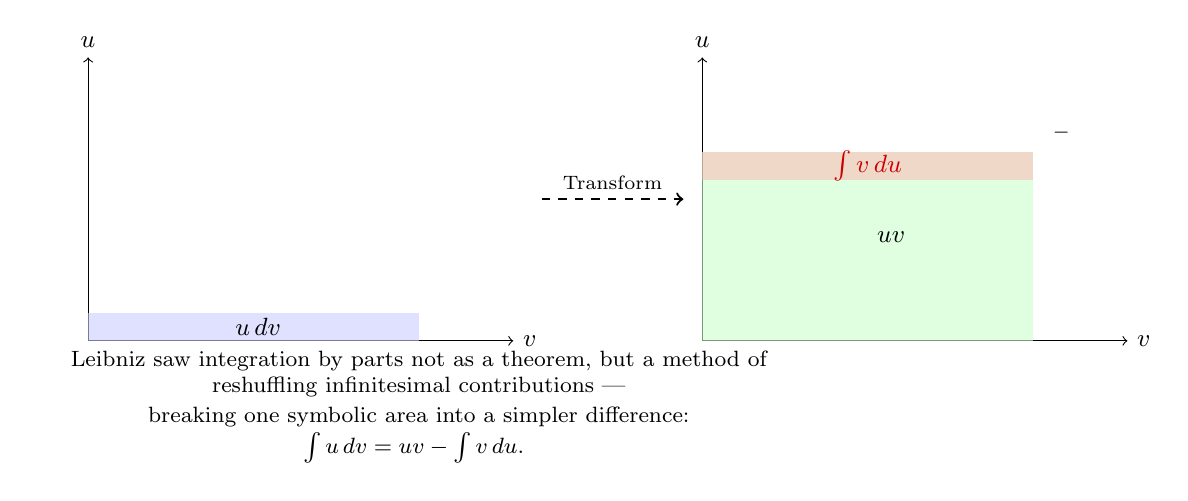
\begin{tikzpicture}[scale=1.2, every node/.style={font=\small}]

  % Axis box for infinitesimal rectangles
  \draw[->] (0,0) -- (4.5,0) node[right] {$v$};
  \draw[->] (0,0) -- (0,3) node[above] {$u$};

  % Rectangle for u dv
  \fill[blue!20,opacity=0.6] (0,0) rectangle (3.5,0.3);
  \node at (1.8,0.15) {$u\,dv$};

  % Dashed arrow to transformed expression
  \draw[->, thick, dashed] (4.8,1.5) -- (6.3,1.5);
  \node[above] at (5.55,1.5) {\scriptsize Transform};

  % Output: uv - ∫v du block
  \begin{scope}[xshift=6.5cm]
    \draw[->] (0,0) -- (4.5,0) node[right] {$v$};
    \draw[->] (0,0) -- (0,3) node[above] {$u$};

    % Highlight uv area (solid block)
    \fill[green!20,opacity=0.6] (0,0) rectangle (3.5,2.0);
    \node at (2.0,1.1) {$uv$};

    % Subtracting integral ∫v du
    \fill[red!30,opacity=0.5] (0,1.7) rectangle (3.5,2.0);
    \node[red!80!black] at (1.75,1.85) {$\int v\,du$};

    % Minus sign
    \node at (3.8,2.2) {\scriptsize $-$};

  \end{scope}

  % Label
  \node at (3.5,-0.7) {
    \begin{minipage}{0.8\linewidth}
      \centering
      {\footnotesize
      Leibniz saw integration by parts not as a theorem, but a method of reshuffling infinitesimal contributions —\\
      breaking one symbolic area into a simpler difference: \quad $\int u\,dv = uv - \int v\,du$.
      }
    \end{minipage}
  };

\end{tikzpicture}
\caption{Leibniz’s idea of integration by parts: transforming one infinitesimal sum into another. Instead of proving a rule, he saw it as a symbolic rearrangement of differentials — from $\int u\,dv$ into $uv - \int v\,du$.}
\end{figure}


To apply this to falling motion, suppose a cannonball has velocity $v$ and time $t$. Multiply both sides of $ds = v\,dt$ by $t$:

\[
t\,ds = t v\,dt
\]

\begin{figure}[H]
\centering
\begin{tikzpicture}[scale=1.3, every node/.style={font=\small}]

  % Axes
  \draw[->] (0,0) -- (5.5,0) node[right] {$t$ (tempus)};
  \draw[->] (0,0) -- (0,3.5) node[above] {$s$ (spatium)};

  % Position curve: s(t) = (1/2)gt^2
  \draw[thick,blue,domain=0:5,smooth,samples=100] plot(\x,{0.35*\x*\x});
  \node[blue] at (4.3,3.1) {\footnotesize $s(t) = \frac{1}{2}gt^2$};

  % Point on the curve
  \coordinate (P) at (3, {0.35*3*3});
  \filldraw[blue] (P) circle (1pt);
  \node[above left] at (P) {\scriptsize $(t,s)$};

  % Tangent line at P
  \draw[->, thick,red] (P) -- ++(1, {0.35*6});
  \node[above right] at ($(P)+(1,0.7)$) {\scriptsize $v = \frac{ds}{dt}$};

  % Vertical line up to P from t-axis
  \draw[dashed] (3,0) -- (P);
  \node[below] at (3,0) {\scriptsize $t$};

  % Horizontal line from P to y-axis
  \draw[dashed] (0,{0.35*9}) -- (3,{0.35*9});
  \node[left] at (0,{0.35*9}) {\scriptsize $s$};

  % Area label (conceptual)
  \node at (2,1.2) {\scriptsize $t\,ds = t v\,dt$};

  % Symbolic infinitesimal rectangle
  \fill[blue!20, opacity=0.5] (3,0) rectangle ++(0.3,{0.35*6*0.3});
  \node[below right] at (3.1,0.1) {\scriptsize $tv\,dt$};

\end{tikzpicture}
\caption{Leibniz’s application of infinitesimals to motion: multiplying both sides of $ds = v\,dt$ by time gives $t\,ds = tv\,dt$. This product represents an infinitesimal contribution to position, scaled by time — the raw material for integration by parts.}
\end{figure}


Now consider the integral of the right-hand side:

\[
\int t v\,dt
\]

\begin{figure}[H]
\centering
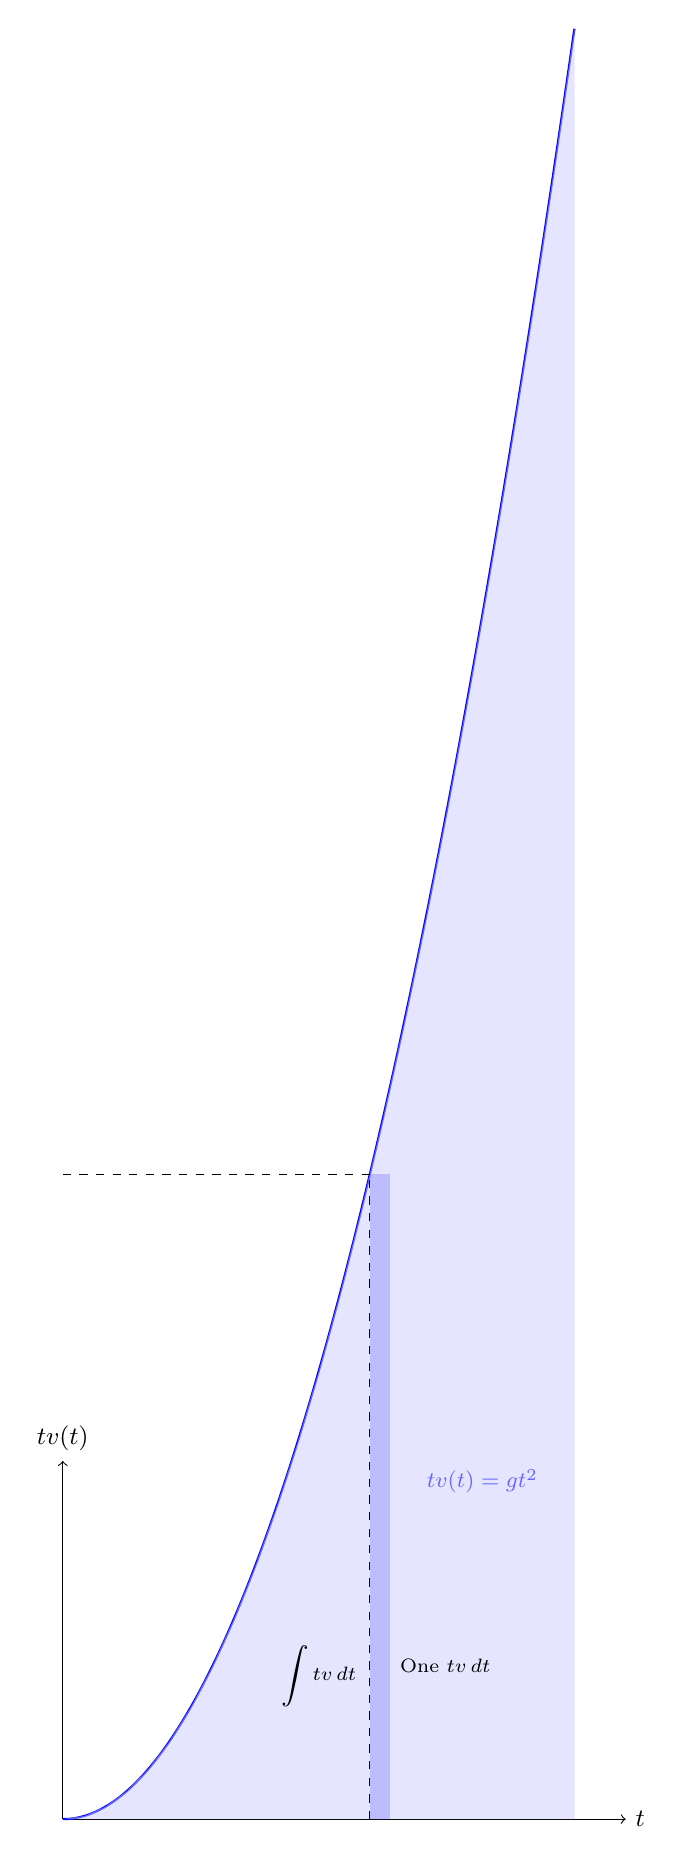
\begin{tikzpicture}[scale=1.3, every node/.style={font=\small}]

  % Axes
  \draw[->] (0,0) -- (5.5,0) node[right] {$t$};
  \draw[->] (0,0) -- (0,3.5) node[above] {$tv(t)$};

  % Curve: t * v(t) = g t^2
  \draw[thick,blue,domain=0:5,smooth,samples=100] plot(\x,{0.7*\x*\x});
  \node[blue] at (4.1,3.3) {\footnotesize $tv(t) = g t^2$};

  % Shaded area under curve (integral)
  \fill[blue!20,opacity=0.5] (0,0) -- plot[domain=0:5] (\x,{0.7*\x*\x}) -- (5,0) -- cycle;

  % Annotation
  \node at (2.5,1.4) {\scriptsize $\displaystyle \int t v\,dt$};

  % Infinitesimal strip at t = 3
  \draw[dashed] (3,0) -- (3,{0.7*3*3});
  \draw[dashed] (0,{0.7*9}) -- (3,{0.7*9});
  \fill[blue!50,opacity=0.4] (3,0) rectangle ++(0.2,{0.7*9});
  \node[right] at (3.2,1.5) {\scriptsize One $t v\,dt$};

\end{tikzpicture}
\caption{The integral $\int t v\,dt$ represents the total accumulation of motion over time, weighted by time itself. It geometrically captures the area under the curve $tv(t) = gt^2$, with each infinitesimal strip representing $tv\,dt$.}
\end{figure}


Let $u = t$, $dv = v\,dt$, so $du = dt$, and $v = s$ (since $ds = v\,dt$). Then, by his rule:

\[
\int t v\,dt = t s - \int s\,dt
\]

\begin{figure}[H]
\centering
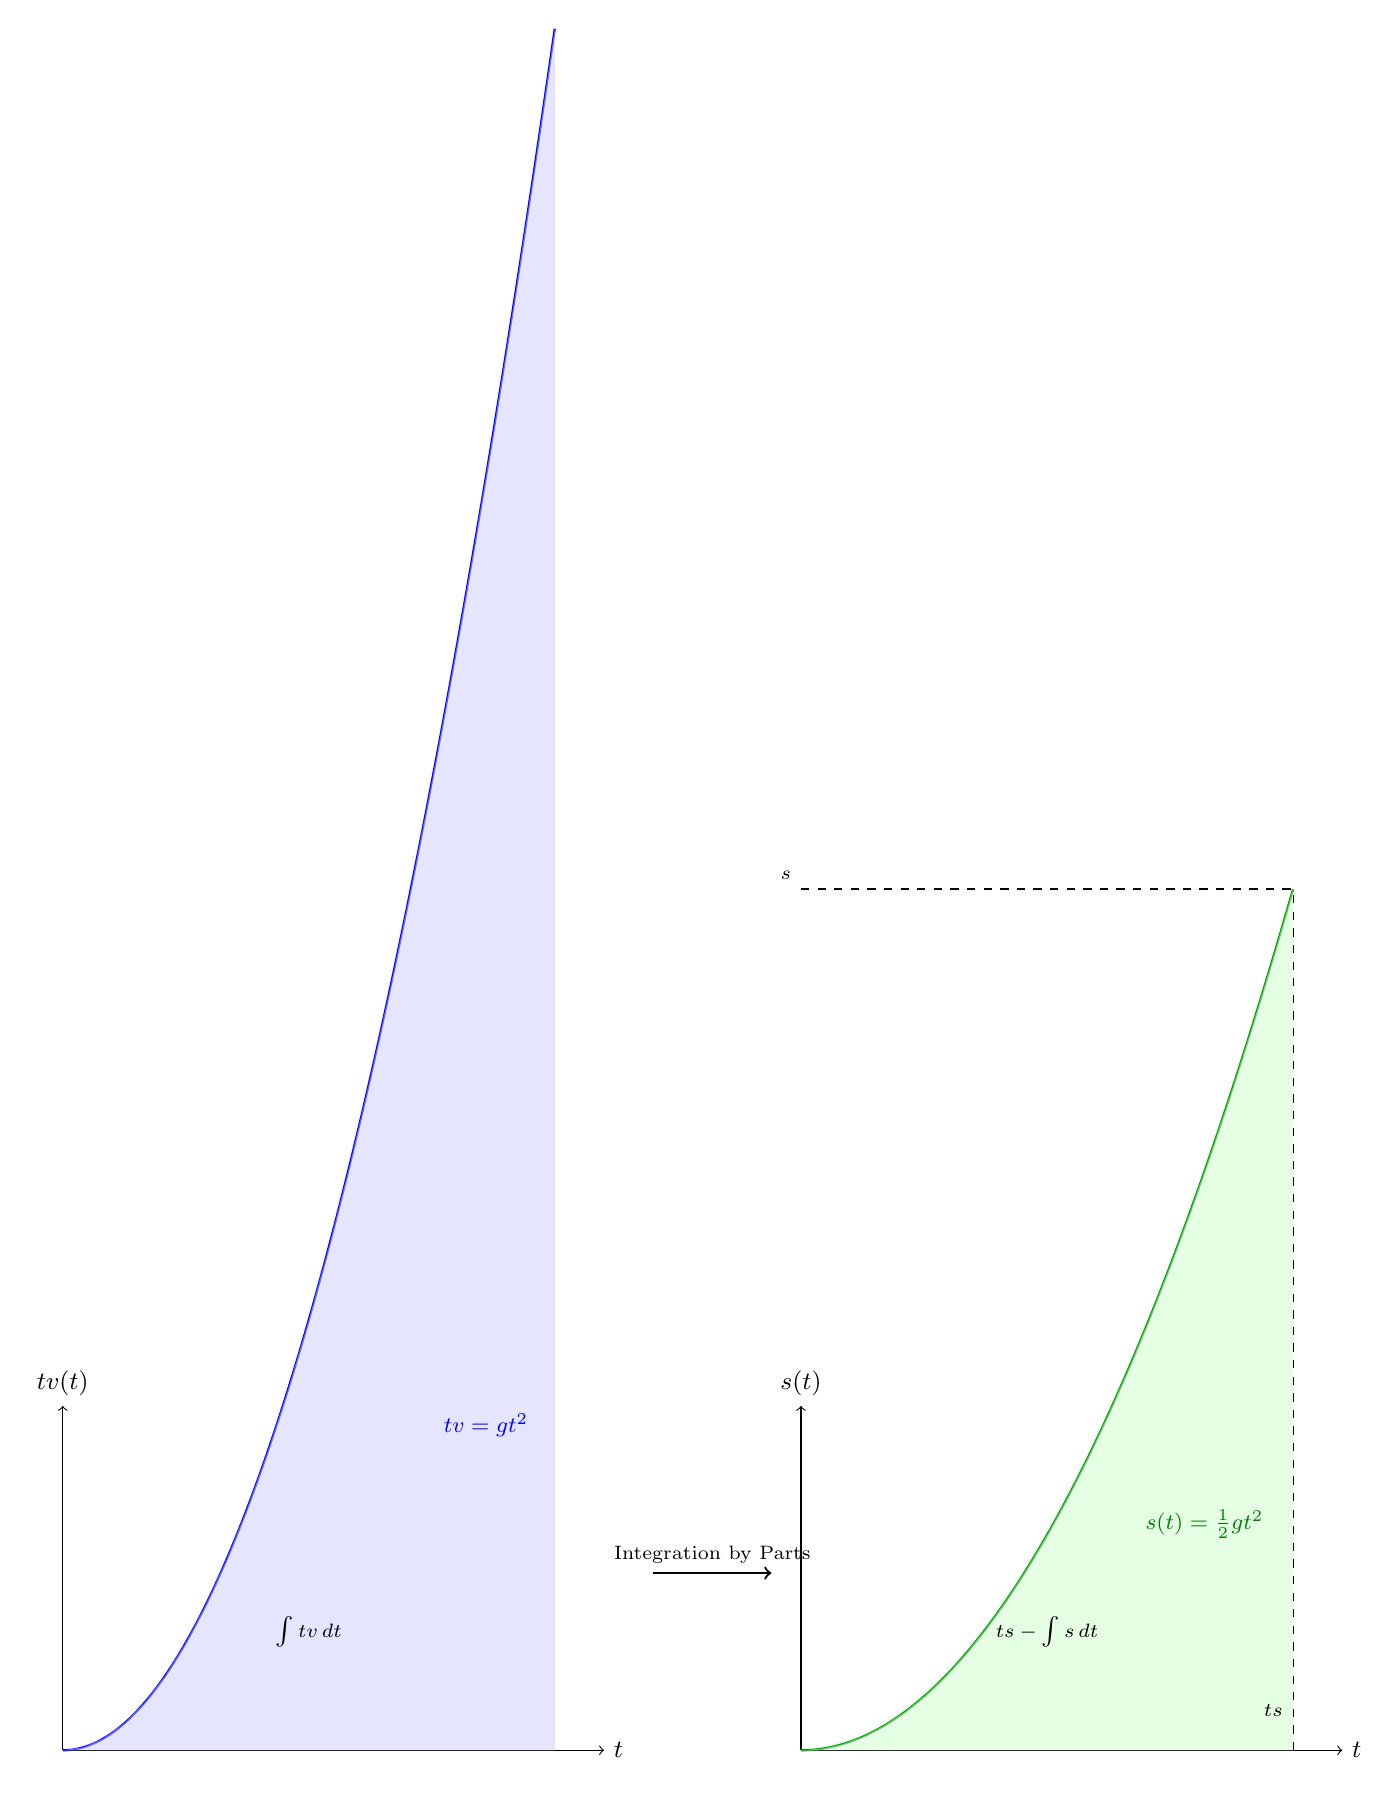
\begin{tikzpicture}[scale=1.25, every node/.style={font=\small}]

  % Left: Original integral (∫t v dt)
  \begin{scope}
    \draw[->] (0,0) -- (5.5,0) node[right] {$t$};
    \draw[->] (0,0) -- (0,3.5) node[above] {$tv(t)$};

    % Curve: tv = gt^2
    \draw[thick,blue,domain=0:5,smooth,samples=100] plot(\x,{0.7*\x*\x});
    \fill[blue!20,opacity=0.5] (0,0) -- plot[domain=0:5] (\x,{0.7*\x*\x}) -- (5,0) -- cycle;
    \node[blue] at (4.3,3.3) {\footnotesize $tv = gt^2$};

    \node at (2.5,1.2) {\scriptsize $\int t v\,dt$};
  \end{scope}

  % Arrow showing transformation
  \draw[->, thick] (6,1.8) -- (7.2,1.8) node[midway, above] {\scriptsize Integration by Parts};

  % Right: Transformed expression ts - ∫s dt
  \begin{scope}[xshift=7.5cm]
    \draw[->] (0,0) -- (5.5,0) node[right] {$t$};
    \draw[->] (0,0) -- (0,3.5) node[above] {$s(t)$};

    % Curve: s = (1/2)gt^2
    \draw[thick,green!60!black,domain=0:5,smooth,samples=100] plot(\x,{0.35*\x*\x});
    \fill[green!20,opacity=0.5] (0,0) -- plot[domain=0:5] (\x,{0.35*\x*\x}) -- (5,0) -- cycle;
    \node[green!50!black] at (4.1,2.3) {\footnotesize $s(t) = \frac{1}{2}gt^2$};

    % Label ts at endpoint
    \node at (4.8,0.4) {\scriptsize $ts$};
    \draw[dashed] (5,0) -- (5,{0.35*25});
    \draw[dashed] (0,{0.35*25}) -- (5,{0.35*25});
    \node[above left] at (0,{0.35*25}) {\scriptsize $s$};

    \node at (2.5,1.2) {\scriptsize $ts - \int s\,dt$};
  \end{scope}

\end{tikzpicture}
\caption{Using integration by parts, Leibniz transformed $\int t v\,dt$ into $ts - \int s\,dt$. For him, this was a way to simplify and symbolically rearrange motion — not geometry, but algebraic bookkeeping with infinitesimals.}
\end{figure}


This gave him a way to understand the accumulation of motion over time in terms of the changing relationship between position and time. Not geometry — but algebraic bookkeeping of motion.

\paragraph{In Leibniz's View:} 

\begin{enumerate}
	\item Galileo provided measurements;
	\item Leibniz gave them algebraic breath;
	\item Infinitesimals were not approximations, but tools of thought;
	\item The integral sign $\int$ stood for “the sum of all $y\,dx$” — a wedge-shaped contribution to motion.
\end{enumerate}

Where Newton used triangles, Leibniz wrote:

\[
dy = f(x)\,dx \quad \Rightarrow \quad y = \int f(x)\,dx
\]

Where Newton argued force from area, Leibniz discovered area from differentials.

\begin{figure}[H]
\centering
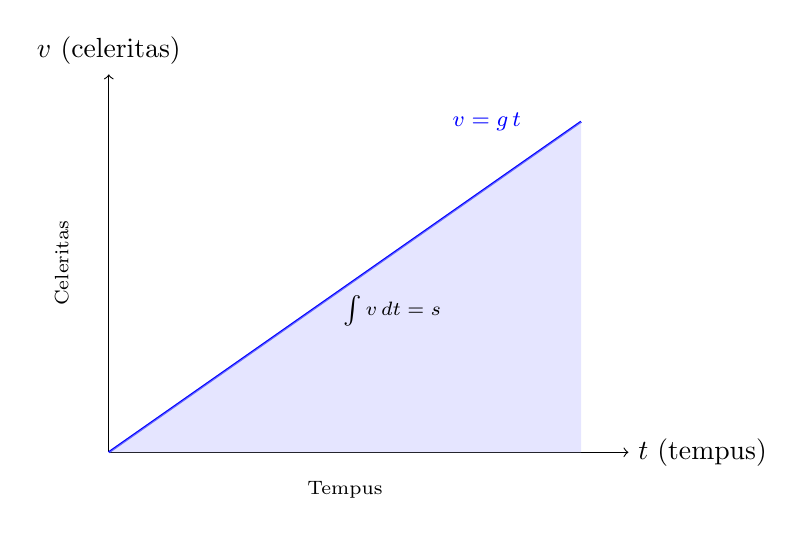
\begin{tikzpicture}[scale=1.2]

  % Axes
  \draw[->] (0,0) -- (5.5,0) node[right] {$t$ (tempus)};
  \draw[->] (0,0) -- (0,4) node[above] {$v$ (celeritas)};

  % Velocity curve: v(t) = g t
  \draw[thick, blue, domain=0:5, samples=100] plot(\x,{0.7*\x});
  \node[blue] at (4,3.5) {\footnotesize $v = g\,t$};

  % Area under curve (shaded)
  \fill[blue!20, opacity=0.5] (0,0) -- plot[domain=0:5] (\x,{0.7*\x}) -- (5,0) -- cycle;

  % Annotations
  \node at (2.5, -0.4) {\scriptsize Tempus};
  \node[rotate=90] at (-0.5, 2) {\scriptsize Celeritas};
  \node at (3,1.5) {\scriptsize $\int v\,dt = s$};

\end{tikzpicture}
\caption{Leibniz’s algebraic conception of motion: the area under the velocity curve represents the distance fallen. Not triangles — but infinitesimals.}
\end{figure}


\begin{tcolorbox}[colback=blue!5!white, colframe=blue!50!black, 
  title={Historical Sidebar: Leibniz—Calculus, Harmony, and the Divine Algorithm}]
  
      \textbf{Gottfried Wilhelm Leibniz} didn’t just co-invent calculus—he invented it as part of a larger metaphysical project: \textbf{to show that the universe was the optimal solution to a divine equation}. For Leibniz, mathematics wasn’t separate from philosophy. It was philosophy, written in symbolic shorthand.
  
      \medskip
  
      His belief in the \textbf{“best of all possible worlds”} had deep theological roots. Leibniz was profoundly influenced by \textbf{Anselm of Canterbury}, the medieval philosopher who defined God as “that than which nothing greater can be conceived.” From that, Leibniz reasoned: if God is maximally perfect and rational, then the world He creates must also reflect that perfection as \textbf{a universe governed by the simplest laws producing the richest variety of outcomes}.
  
      \medskip
  
      This obsession with harmony and optimization laid the philosophical foundation for what would become variational calculus. Leibniz saw nature as a system that doesn’t waste effort—it minimizes and balances, like a cosmic engineer working with divine efficiency.
  
      \medskip
  
      His version of calculus focused on infinitesimals—quantities so small they straddle the line between something and nothing. These weren’t just technical tools. They reflected his belief that \textbf{all change happens gradually, rationally, and with purpose}. Nature, he argued, doesn’t leap; it glides.
  
      \medskip
  
      Even his notation—those now-familiar \texttt{dx} and \texttt{dy} symbols—reflected a vision of the universe as a flowing, continuous, and infinitely divisible system. To Leibniz, calculus was a kind of \textbf{divine syntax}: a universal language that could express not just motion and mechanics, but logic, theology, and metaphysical truth. In short, Leibniz wasn’t just trying to solve math problems. He was trying to read the mind of God... with math.
  
      \medskip
  
      \textbf{Quote from Leibniz (1686):}
      \begin{quote}
      “The present is pregnant with the future; the future could be calculated from it, if we had sufficient knowledge of all causes.”
      \end{quote}
  
  
  \end{tcolorbox}
  







---
